%\section[Naslov sekcije u sadržaju][Kratki naslov sekcije]{Naslov sekcije}
\chapter[Teorija grafova][TG]{Teorija grafova}
\section[Općenito o grafovima][Općenito o grafovima]{Općenito o grafovima}

\begin{defn}
\textbf{Usmjeren težinski graf} je dan kao trojka $G = ( \mathcal{V}, \mathcal{E}, \{ w_{j,k} \}_{j,k=1}^{n} )$, gdje je $\mathcal{V} = \{v_1,...,v_n\}$ neprazan skup vrhova, $\mathcal{E} \subset \mathcal{V} \times \mathcal{V} $ skup bridova i $w_{j,k} \geq 0 $ su težine bridova. $w_{j,k} > 0$  akko $(v_j,v_k) \in \mathcal{E}$. 
Kažemo da su luk $e \in \mathcal{E}$ i vrh $v \in \mathcal{V}$ \textbf{incidentni} ako luk $e$ izlazi iz vrha $v$.
\end{defn}
\begin{rem}
    Ova definicija se može primjeniti i za neusmjereni graf. U tom slučaju je Laplaceova matrica grafa simetrična i pozitivno definitna.
    Za usmjeren graf je općenito: $w_{j,k} \neq w_{k,j}$.
    Često ćemo za usmjereni graf reći \emph{digraf}
\end{rem}

\begin{defn}
Neka je dan skup \textbf{susjeda} vrha $v_i$ kao $\mathcal{N}_i = \{j : (v_j,v_i) \in \mathcal{E} \:\}$.
    Za usmjereni graf G definiramo \textbf{Laplaceovu matricu} $L \in \R^{n \times n}$ kao:
    $$L = \left[ l_{ij} \right], \quad l_{ij} = 
    \begin{cases}
        - w_{ij}, & j \in \mathcal{N}_i, \\
        \sum\limits_{k\in \mathcal{N}_i} w_{ik}, & j=i,\\
        0, & \text{inače}\\
    \end{cases}$$
\end{defn}
\begin{rem}
    Ekvivalento, za graf $G$ mogu se uvesti \textbf{matrica susjedstva} $A$ i \textbf{\emph{in-degree} matrica} $D$. $A$ se definira kao $n \times n$ matrica čiji su stupci i retci indeksirani po vrhovima te na poziciji $a_{ij} = w_{ij}$ ako je $(v_i, v_j) \in \mathcal{E}$, a nula inače. $D$ se definira kao $n \times n$ dijagonalna matrica koja na poziciji $d_{ii}$ ima sumu $i$-tog retka matrice $A$. Tada se Laplacian grafa $G$ definira kao $L = D-A$.
\end{rem}
Laplaceova matrica na dijagonali prikazuje stupanj pojedinog vrha a na vandijagonalnim elementima su prikazane težine pojedinog brida.
\begin{exa}
    Ilustrirajmo Laplaceovu matricu na jednostavnom primjeru grafa
$G = \{ \mathcal{V}, \mathcal{E}\}$, gdje su $\mathcal{V} = \{1,2,3\}$ i $\mathcal{E} = \{(1,2), (3,2), (2,1)\}$. Tada je $$L = \begin{bmatrix}
    1 & -1 & 0 \\
    -1 & 2 & -1 \\
    0 & 0 & 0\\
\end{bmatrix}$$
\end{exa}
Kao što vidimo, za usmjeren graf Laplaceova matrica $L$ ne mora biti simetrična.

Općenito za grafove uvodimo pojam \emph{povezanosti} i \emph{komponenti povezanosti}. Za definiciju povezanosti nužno je uvesti pojmove \emph{šetnje} i \emph{puta.} slično kao u \cite{Diskretna} i \cite{Operacijska}.
\begin{defn}
    \textbf{Šetnja} je niz vrhova i njima incidentnih lukova $v_{i_1} e_{j_1} v_{i_2} \dots v_{i_{N-1}} e_{j_{N-1}} v_{i_N}$. Luk $e_{j_k}$ nazivamo \textbf{direktnim} lukom šetnje ako je $(v_{i_k},v_{i_{k+1}}) \in \mathcal{E}$, a ako je $(v_{i_{k+1}},v_{i_k}) \in \mathcal{E}$ onda ga nazivamo \textbf{obrnutim}. Direktni put između vrhova $v_i$ i $v_j$ označavat ćemo sa $v_i \dipath v_j$.\\
    \textbf{Put} je šetnja u kojoj su svi vrhovi osim eventualno prvog i zadnjeg međusobno različiti.\\ 
    \textbf{Ciklus} je put u kojem su prvi i zadnji vrh jednaki.\\
    Kažemo da je graf \textbf{povezan} ako za svaka dva vrha postoji put među njima.
\end{defn}
\begin{defn}
    Podgraf $(\mathcal{V}', \mathcal{E}')$ grafa $(\mathcal{V}, \mathcal{E})$ je graf u kojemu su $\mathcal{V}' \subset  \mathcal{V}$ i $\mathcal{E}' \subset \mathcal{E}$ te vrijedi da su za svaki brid $e \in \mathcal{E'}$ njegovi vrhovi $v_{e_1},v_{e_2} \in \mathcal{V}'$.
    
\end{defn}

Za neusmjereni graf postoji veza između broja komponenti povezanosti i jezgre Laplaceove matrice \cite{smola2003kernels}:
\begin{thm}
    Neka je dan neusmjeren graf $G$ te neka je $L$ njegova Laplaceova matrica. Tada je algebarska kratnost svojstvene vrijednosti nula jednaka broju komponenti povezanosti grafa G.
\end{thm}
Drugim riječima, ako je graf $G$ povezan tada je nula su spektru od $L$ i ima algebarsku kratnost 1.


\section[Pobliže o usmjerenim grafovima][Pobliže o usmjerenim grafovima]{Pobliže o usmjerenim grafovima}
Općenito se Laplaceova matrica $L$ usmjerenog grafa $G$ može zapisati u formu $M = D-DS$ gdje je $D$ prikladno odabrana nenegativna dijagonalna matrica, a $S$ je stohastička. Općenito za bilo koju takvu matricu $M = D-DS$ vrijedi da su algebarska i geometrijska kratnost svojstvene vrijednosti nula jednake \cite{DiGraph_Kernel}. Štoviše, postoji veza između jezgre i strukture grafa.
\begin{defn}
    \begin{enumerate}[i.)] Neka je $G$ usmjeren težinski graf.
  \item $G$ je \textbf{jako povezan} ako za svaki uređeni par vrhova $(v_i, v_j)$ postoji direktan put $v_i \dipath v_j$.
  \item $G$ je \textbf{jednostrano (unilaterally) povezan} ako za svaki uređeni par vrhova $(v_i, v_j)$ postoji direktan put $v_i \dipath v_j$ ili $v_j \dipath v_i$
  \item $G$ je \textbf{slabo povezan} ako je pripadni neusmjereni graf povezan.
  \item $G$ \textbf{nije povezan} ako nije slabo povezan.
\end{enumerate}
\end{defn}
Podrgaf koji je jako povezan nazivamo \textbf{jako povezana komponenta}.
Proučavanje nepovezanog grafa se svodi na proučavanje svake komponente zasebno. Stoga su slabo povezani digrafovi najopćenitija struktura za proučavanje.
Potrebno je uvesti dodatne pojmove kako bi se opisalo pojedine podrgafove.

\begin{defn}Definiramo pojmove
    \begin{enumerate}[i.)]
        \item Za vrh $i \in \mathcal{V}$ definiramo \textbf{dostižni skup (reachable set)} $R(i) = \{ j \in \mathcal{V} : i \dipath j \:\}$.
        \item \textbf{Doseg} $R$ je najveći dostižni skup ili najveći jednostrano dostižni skup.
        \item \textbf{Kabal (cabal)} $B \subset R$ je skup vrhova iz kojih se dostiže cijeli $R$. Ako $R$ sadrži samo jedan vrh, taj vrh nazivamo \textbf{korjen}.
        \item \textbf{Ekskluzivni dio} $H \subset R$ je skup vrhova iz $R$ koji ne "vide" vrhove iz drugih dosega.
        \item \textbf{Zajednički dio} $C \subset R$ je skup svih vrhova iz $R$ koji "vide" vrhove iz drugih dosega.
    \end{enumerate}
\end{defn}

\begin{figure}[H]
    \centering
    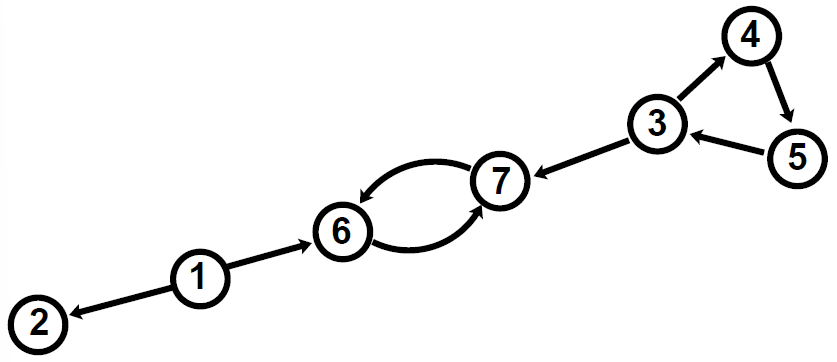
\includegraphics[width=0.5\textwidth]{digrafPrimjer.png}
    \caption{Primjer grafa $G_1$}
    \label{fig:Pr1}
\end{figure}

\begin{exa}
    Pogledajmo primjer grafa $G_1$ sa slike \ref{fig:Pr1} preuzetoga iz \cite{DiGraphReach}:  
Ovdje svaki doseg ima jedan neprazan kabal. Ovaj graf ima dva dosega $R_1 = \{1,2,6,7\}$ i $R_2 = \{3,4,5,6,7\}$ (vidi sliku \ref{fig:Pr1_dosezi}). Ekskluzivni dijelovi su $H_1 = \{ 1,2\}$, $H_2 = \{3,4,5\}$. Kabali su $B_1 = \{1\}$ $B_2 = \{3,4,5\}$. Zajednički dijelovi su $C_1 = C_2 = \{6,7\}$
\end{exa}
\begin{figure}[H]
    \centering
    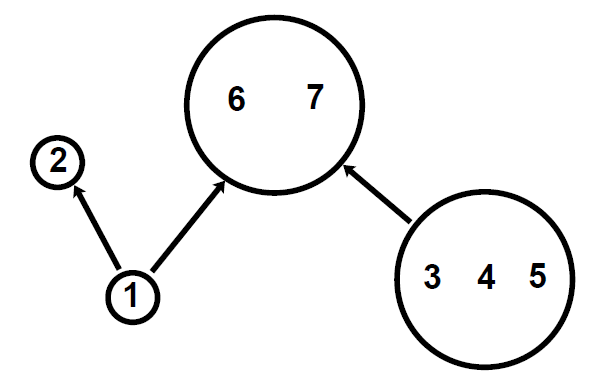
\includegraphics[width=0.5\textwidth]{digrafPrimjer_reaches.png}
    \caption{Dosezi grafa $G_1$}
    \label{fig:Pr1_dosezi}
\end{figure}

Postoji veza između jezgre Laplaceove matrice digrafa $L$ i broja dosega digrafa $G$ \cite{DiGraph_Kernel}:
\begin{thm} %TM 4.6
    Neka je dan digraf G. Tada su algebarska i geometrijska kratnost svojstvene vrijednosti 0 jednake broju dosega. 
\end{thm}
\clearpage
\section[Grafovi u testu][Nekoliko tipova grafova korištenih za testiranje]{Neki tipovi grafova}
U našem radu koristili smo nekoliko vrsta grafova koje nudi Python biblioteka networkx
\subsection{gn\_graph}

